\documentclass[a4paper]{article}
\usepackage[spanish]{babel}
\usepackage[utf8]{inputenc}
\usepackage{graphicx}
\usepackage{float}

\usepackage{biblatex}
\addbibresource{final2.bib}

\title{Proyecto Final}
\author{José Soto García}
\begin{document}
\maketitle
\begin{abstract}
https://github.com/sotowe/proyecto$\_$final\\\\
palabras clave: Proyecto, Final. 
\end{abstract}
\section{Introducción}
algo algo algo algo algo algo algo algo algo algo algo algo algo algo algo algo algo algo algo algo algo algo algo algo algo algo algo algo algo algo algo algo algo algo algo algo algo algo algo algo\cite{bransden2000},\cite{krane1988}, algo algo algo algo algo algo algo algo algo algo algo algo algo algo algo algo algo algo algo algo algo algo algo algo algo algo algo algo algo algo algo algo algo algo algo algo algo algo algo algo algo algo algo algo algo algo algo algo algo algo algo algo algo algo algo algo algo algo algo algo algo algo algo algo algo algo algo algo algo algo algo algo algo algo algo algo algo algo algo algo \cite{bransden2000}, \cite{tipler2007physics}.
\section{Estado del arte}
algo algo algo algo algo algo algo algo algo algo algo algo algo algo algo algo algo algo algo algo algo algo algo algo algo algo algo algo algo algo algo algo algo algo algo algo algo algo algo algo \cite{kittel1963quantum}.
\section{Imágenes y tablas}
Incluimos en esta sección algunas imágenes y tablas:
\begin{table}[h]
\begin{center}
\begin{tabular}{|l|l|}
\hline
Algo & Algo \\
\hline \hline
Algo & Algo \\ \hline
Algo & Algo \\ \hline
Algo & Algo \\ \hline
\end{tabular}
\caption{Tabla simple.}
\label{tabla:sencilla}
\end{center}
\end{table}

\begin{figure}[H]
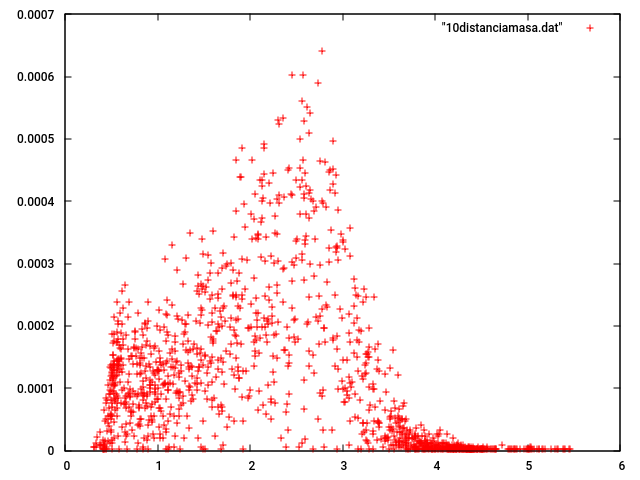
\includegraphics[width=0.9\textwidth]{10distanciamasa.png}
\caption{Imagen}
\end{figure}
\section{Fórmulas}
Escribiremos algunas fórmulas sencillas:
$$A=\sum_{m,n,p}C(\rho_{mnp})e^{-i\triangle k\cdot(ma+nb+pc)}$$
$$\oint{EdS}= \frac{1}{\epsilon_0}\int_V{\rho dV} $$
\newpage
\printbibliography

\end{document}